\section{Problem Setup}
\label{sec:problemSetup}
In this section, we present the setup in which we study the throughput/power trade-off and its effect on control performance. 
We developed a $1/10^{th}$ scale autonomous car equipped with a front facing monocular camera.
The car runs the Vanishing Point algorithm \cite{VP1,VP2} and a feedback controller to navigate a corridor and stay in its middle.
The car is equipped with a front facing monocular camera which feeds image frames to the vanishing point algorithm for processing.
The computation platform on board the car is a Nvidia Jetson, which has a quad-core ARM CPU and a 192 core Nvidia Tegra GPU.


\subsection{Vanishing point for corridor navigation}

The Vanishing Point algorithm (VP) \cite{VP1} has been used extensively in indoor settings for navigating corridors autonomously \cite{VP2, VP3} and for outdoor lane detection \cite{gallagher2002ground}.
For each image frame, the algorithm outputs the horizontal distances $x_v$ of the vanishing point and $x_m$ of the middle point from the center of the frame. 
The vanishing point is the intersection point of any two parallel lines in the environment, and the middle point indicates the center of the corridor. 
These two measurements are used by the feedback controller to center the robot in the corridor and align it with the walls. 
It does so by driving the abcissa $x_v$ and $x_m$ to zero. 
See Fig. \ref{fig:juicyj}.
Figure \ref{fig:vp_viz} shows a sample processed frame.

\begin{figure}[t]
\centering
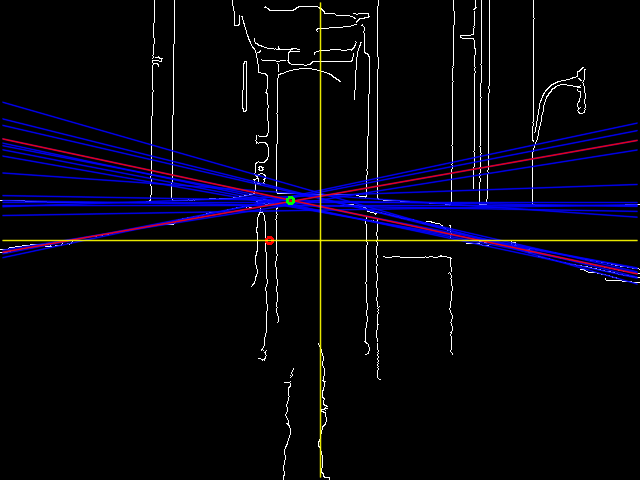
\includegraphics[width=0.46\textwidth]{Figs/vpmpimages/image_23_-30_-51.png}
\caption{Visualization of the Vanishing point algorithm. The green (upper) dot shows the vanishing point while the red (lower) dot shows the middle point.}
\label{fig:vp_viz} %diff freq same assignment}
\end{figure}

 We define \textit{throughput} as the update rate of VP, which is the inverse of its execution time. 
 The faster VP executes, the better the control performance of the closed loop system since the controller sees a small delay. 
 Hence, throughput acts as a proxy for control performance. 
 In most implementations, the perception algorithm is always run at its maximum possible throughput to subject the controller to the smallest possible delays.
 This neglects the power consumed by the computation platform.
 In many autonomous systems, power draw from the computation platform is a significant concern; e.g., in our robot, the Jetson and drive motors are powered by separate energy sources.
 So while we would want to subject the controller to a small delay (operate the perception algorithm at a high throughput), we would also like to minimize the power draw from the computation platform in order to maximize the operating time of the system. 
  

\subsection{Exploiting hardware knobs to trade-off power and throughput}

In order to trade-off computation power and throughput of the perception algorithm, we rely on the insight that the GPU can execute some tasks faster than a CPU, albeit at a greater power cost.
Also, executing a task at a higher frequency (on either CPU or GPU) increases throughput, but again at a greater power cost.
Thus, in our implementation, we found that running VP on the CPU alone resulted in a low throughput (~8Hz) and low power consumption (~5.2W). 
On the other hand running it on the GPU allowed us to get a throughput in excess of 20Hz, but resulted in a power consumption of over 7W. 
In this section, we describe how to divide VP into tasks and profile VP's performance as we vary the execution frequencies of these tasks and their scheduling on either CPU or GPU.
These tasks are (see Fig. \ref{fig:vanishing}):

\begin{itemize}
\item Blur: A Gaussian blur is applied on the image for de-noising.
\item Edge detection: We use the Canny Edge detector to find edges in the image.
\item Hough Transform: used to detect straight lines in the image.
\item RANSAC: used to select the parallel straight lines that best describe the sides of the corridor. These lines intersect in the image plane at the Vanishing Point.
\end{itemize}

We can schedule any of these tasks to be run on either the CPU or the GPU as shown in Fig. \ref{fig:vanishing}.
Let $\sigma \in \Sigma$ denote a given schedule, where 
\[\Sigma=\{\text{CCC, CCG, CGC, CGG, GCC, GCG, GGC, GGG}\} \]
For example, schedule $\sigma=$ CCG means that the Blur task is done on the CPU, the Edge detection is done on the CPU and the Hough Transform is done the GPU, and so on.
Since RANSAC took a negligible amount of time compared to the other tasks, we always execute it on the CPU.
In addition, we can change the CPU and GPU frequencies during run-time, resulting in different execution times and power consumption for the Jetson. 
Let $F_c$ and $F_g$ be the frequencies of the CPU and the GPU respectively. 

The hardware level knobs to trade-off throughput and computation power for an execution of the vanishing point algorithm are now $\sigma$, $F_c$ and $F_g$. 
The throughput and computation power, functions  of all three knobs, are denoted by $T(\sigma,F_c,F_g)$ and $P(\sigma,F_c,F_g)$ respectively.


\begin{figure}
	\centering
	\includegraphics[scale=0.3]{Figs/vanishing}
	\caption{The vanishing point algorithm with components running on either CPU or GPU at various frequencies, resulting in different power consumptions and execution times.}
	\label{fig:vanishing}		
\end{figure}

\subsection{Problem statement}
The problem we solve is that of picking the best operating mode ($\sigma$, $F_c$ and $F_g$) for the perception algorithm VP in order to minimize computation power $P(\sigma,F_c,F_g)$ without overly affecting the closed loop control performance of the system, quantified by the throughput $T(\sigma,F_c,F_g)$. 
